\clearpage\subsection{Uploading Music}

\noindent\makebox[\textwidth]{
\begin{tabularx}{1.5\textwidth}{XX}
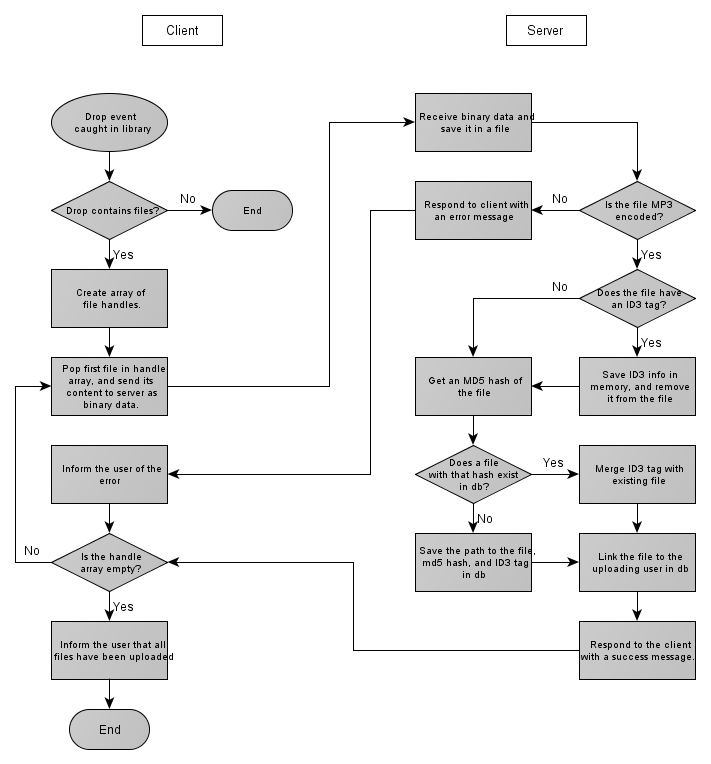
\includegraphics[scale=0.709]{design/figures/uploadflow}
\end{tabularx}}

Uploading music to your library is probably the most crucial functionality in our project. For this reason it is important that
it requires as little effort from the user as possible.

On the client, the only input we need is the actual drop of what the user wants uploaded. And as seen, should there be errors in the
upload, there will be a small notice to the user, and the process will resume for any remaining files without requiring input. This
solution was chosen since there is a high risk that when a user uploads an album, some non-music files will be uploaded (album
 picture, overhead from local music players, etc.).

On the server a bit more is going on. As there is no reason to spend resources processing non-music files it first checks if the file is
actually encoded as an mp3, and if not the server just requests the next file from the client.

If the file is an mp3, it is checked wether it has an ID3 tag\cite{ONeill10}. The reason for checking and removing this at this point in
the process is that when we hash the file we are not interested in the ID3 information, as we just want to check wether the sound file is
the same.

When file processing is done, a database entry is made to link it to the user, and the next file is requested. The reason the files
should be sent one at a time is that it reduces the size of individual network packages. One advantage of this, is that should the
connection between server and client be unexpectedly terminated while an upload is in progress, only that file will be lost, and not the
entire upload.